% This is samplepaper.tex, a sample chapter demonstrating the
% LLNCS macro package for Springer Computer Science proceedings;
% Version 2.21 of 2022/01/12
%
\documentclass[runningheads]{llncs}
%
\usepackage[T1]{fontenc}
\usepackage{graphicx}

\usepackage[utf8]{inputenc} % allow utf-8 input
\usepackage[T1]{fontenc}    % use 8-bit T1 fonts
\usepackage{hyperref}       % hyperlinks
\usepackage{url}            % simple URL typesetting
\usepackage{booktabs}       % professional-quality tables
\usepackage{amsfonts}       % blackboard math symbols
\usepackage{nicefrac}       % compact symbols for 1/2, etc.
\usepackage{microtype}      % microtypography
\usepackage{xcolor}         % colors
\usepackage{graphicx}
\usepackage{amsmath}
\usepackage{wrapfig}
\usepackage[toc,page]{appendix}
\usepackage{amssymb}
\usepackage{bbding}
\usepackage{multirow}
\usepackage{paralist}
\usepackage{mdframed}
\usepackage{framed}
\usepackage{longtable}
\usepackage[table]{xcolor}

% \newcommand{\manabe}[1]{\textcolor{cyan}{[manabe: #1]}}
% \newcommand{\shibata}[1]{\textcolor{blue}{[shibata: #1]}}
\newcommand{\manabe}[1]{\textcolor{black}{#1}}
\newcommand{\shibata}[1]{\textcolor{black}{#1}}

\definecolor{lightgreen}{RGB}{230,255,230}

% Used for displaying a sample figure. If possible, figure files should
% be included in EPS format.
%
% If you use the hyperref package, please uncomment the following two lines
% to display URLs in blue roman font according to Springer's eBook style:
%\usepackage{color}
%\renewcommand\UrlFont{\color{blue}\rmfamily}
%
\begin{document}
%
\title{
% Sign-to-Speech Prosody Transfer
Sign-to-Speech Prosody Transfer \\
via Sign Reconstruction-based GAN
% SignRecGAN: Sign-to-Speech Prosody Transfer via Sign Reconstruction
}
%
%\titlerunning{Abbreviated paper title}
% If the paper title is too long for the running head, you can set
% an abbreviated paper title here
%
\author{Toranosuke Manabe\orcidID{0009-0003-5058-7735} \and
Yuto Shibata\orcidID{0009-0005-4225-3887} \and
Shinnosuke Takamichi\orcidID{0000-0003-0520-7847} \and
Yoshimitsu Aoki\orcidID{0000-0001-7361-0027}
}
%
\authorrunning{T. Manabe et al.}
% First names are abbreviated in the running head.
% If there are more than two authors, 'et al.' is used.
%
\institute{Keio University, Yagami Campus, Yokohama Kanagawa 223-8522, Japan
\email{torapira@keio.jp},
\email{yuto19990715@gmail.com},
\email{shinnosuke\_takamichi@keio.jp},
\email{aoki@elec.keio.ac.jp}
}
%
\maketitle              % typeset the header of the contribution
%
\begin{figure}[ht]
\centering
\vspace{-6mm}
\centerline{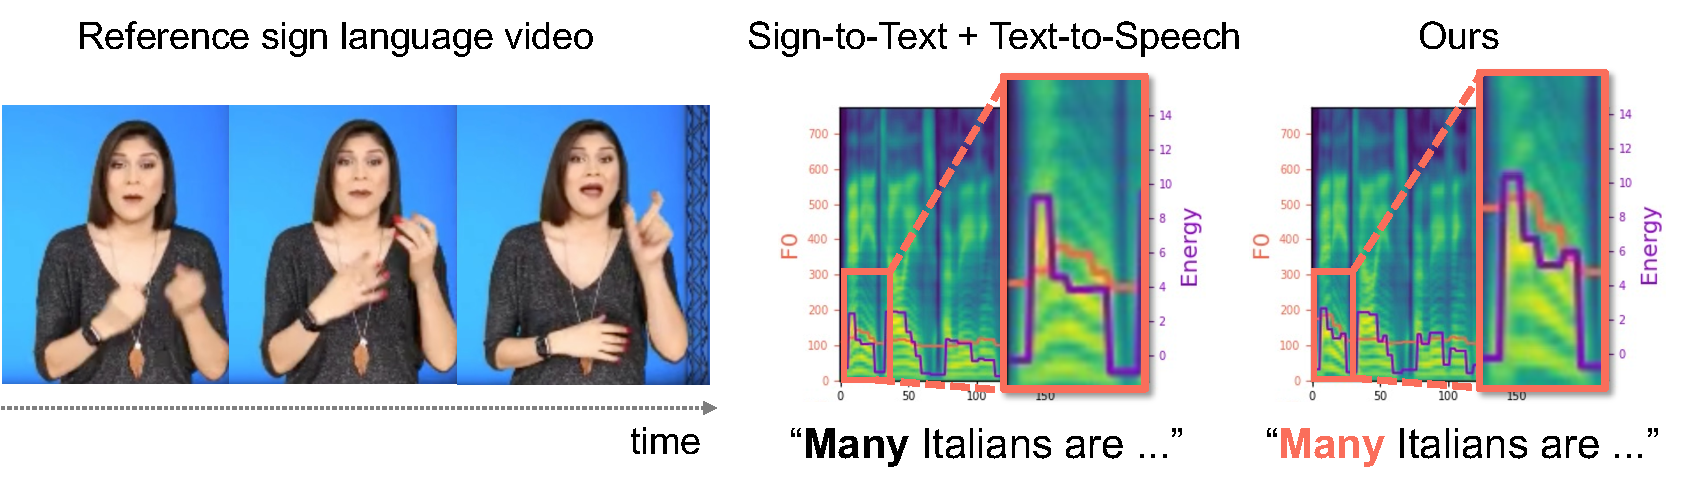
\includegraphics[width=\linewidth]{assets/heading.pdf}}
\vspace{-5mm}
\caption{
% We propose S2PFormer for \emph{Sign-to-Speech Prosody Transfer} task. 
% Our key idea is to directly transfer the sign language prosody into speech synthesis by ensuring that the prosodic cues of the sign language can be reconstructed from the synthesized speech.
In the reference sign language video (left), the first phrase, ``many Italians,'' is emphasized through rapid hand movements and facial expressions. The two-stage baseline (middle) fails to reflect this prosody, whereas our approach (right) successfully captures the emphasis on ``many.''}
\vspace{-8mm}
\label{fig:pipeline}
\end{figure}

\begin{abstract}
% Sign language is a vital means of communication for individuals with hearing impairments.
Deep learning models have improved sign language-to-text translation and made it easier for non-signers to understand signed messages. 
When the goal is spoken communication, a naive approach is to convert signed messages into text and then synthesize speech via Text-to-Speech (TTS).
However, this two-stage pipeline inevitably treat text as a bottleneck representation, causing the loss of rich non-verbal information originally conveyed in the signing. 
To address this limitation, we propose a novel task, 
\emph{Sign-to-Speech Prosody Transfer}, 
which aims to capture the global prosodic nuances expressed
in sign language and directly integrate them into synthesized speech. 
A major challenge is that aligning sign and speech requires expert knowledge, 
making annotation extremely costly and preventing the construction of large parallel corpora. 
To overcome this, we introduce \emph{SignRecGAN}, 
a scalable training framework that leverages unimodal datasets 
without cross-modal annotations through adversarial learning 
and reconstruction losses. 
Furthermore, we propose \emph{S2PFormer}, 
a new model architecture that preserves the expressive power of existing TTS models 
while enabling the injection of sign-derived prosody into the synthesized speech.
Extensive experiments demonstrate that the proposed method can synthesize speech that faithfully reflects the emotional content of sign language, thereby opening new possibilities for more natural sign language communication. Our code will be available upon acceptance.

\keywords{
Sign language 
\and Prosody transfer
% \and Speech synthesis.
\and Multi-modal learning.
}
\end{abstract}

\section{Introduction}
\label{sec:introduction}
%-----------------------------------
Sign language serves as a principal means of communication for individuals with hearing impairments.
Translating between sign language and spoken language is, 
however, a complex task that typically requires specialized knowledge.
Recently, sign-to-text translation methods based on deep learning have been developed~\cite{Camgoz_2020_CVPR,zhang2023sltunet,lin-etal-2023-gloss,Gong_2024_CVPR,NEURIPS2024_ced76a66}.
These methods substantially simplify the process of bridging sign language and spoken language.

\manabe{
However, existing studies are all limited to sign-to-text conversion.
Therefore, to convert sign language into speech using current methods, 
one must rely on a decoupled process consisting of sign-to-text and text-to-speech (TTS). 
In this pipeline, the intermediate text inevitably becomes a bottleneck, 
causing non-verbal information present in the original sign, such as tension and emphasis, to be lost.
Omitting these elements can result in speech that lacks expressiveness.
}
% Nonetheless, most existing sign language translation techniques focus on 
% converting sign language to text, rather than directly synthesizing speech.
% Consequently, obtaining speech from sign language models~\cite{Zhou2020Sign-to-speech,Sharma2020Sign,Dangat2023Sign,Ojha2020Sign,R2022Indian} generally involves a 2-stage pipeline --- sign-to-text followed by text-to-speech.
% This approach introduces a significant shortcoming: because only text is used as the intermediate representation, the rich prosodic information inherent in sign language (e.g., emotion and emphasis~\cite{Brentari2015The}) is lost.
% Omitting these elements can result in speech that lacks expressiveness.

To fill this gap, we propose a novel task,
\emph{sign-to-speech prosody transfer}
to incorporate the global prosody embedded in sign language into speech synthesis process.
\manabe{
This task can be seen as an extension of existing 
cross-lingual prosody transfer~\cite{swiatkowski23_interspeech}.
While the existing task aims to transfer prosody 
from source spoken language to target one, 
our task transfers from source \textit{sign language}.
% This task is one of the classes of cross-lingual prosody transfer~\cite{},
% which aims to transfer global prosody style of the speech of source language into the speech of target language.
}

\shibata{
Here, translating between sign language and speech requires highly specialized expertise.
Consequently, constructing large-scale paired datasets is much more difficult than in other multi-modal transformation problems such as text-to-image~\cite{Rombach_2022_CVPR}, where massive paired data are readily available.
}
\manabe{ 
Moreover, both sign language and speech are time-series data, 
and creating annotations that take their temporal alignment into account is even more challenging.
}
% Achieving this task entails overcoming three major difficulties.
% (i) Speech prosody itself is complex, making it extraordinarily challenging to learn its underlying distribution accurately.
% (ii) Constructing a paired dataset that precisely annotates both sign language and speech requires extensive expertise, and existing datasets remain limited in size.
% (iii) No established technique directly aligns prosodic features between sign language and speech, and the relationship itself is highly intricate and subtle.

% \manabe{
% To address these challenges, in this paper, we propose \emph{SignRecGAN}, 
% a method for converting global prosody from sign language into speech 
% using separate \emph{unimodal datasets} of sign and speech,
% together with \emph{S2PFormer}, a model architecture designed for this task. 
% SignRecGAN combines adversarial learning with reconstruction losses,
% \emph{SignRec loss} (Sign Reconstruction loss) and \emph{ProMo loss} (Prosody-Motion alignment Loss), which recover motion information of sign language from speech, 
% thereby enabling the motion expressed in signing to be reflected in natural-sounding speech. 
% S2PFormer augments a pretrained TTS model 
% with a carefully designed additional cross-attention branch, 
% achieving speech synthesis that incorporates sign information 
% while preserving the original high speech quality.
% }
\shibata{
To address these challenges, in this paper we propose \emph{SignRecGAN}, 
a method for converting global prosody from sign language into speech 
using separate \emph{unpaired unimodal datasets} of sign and speech,
together with \emph{S2PFormer}, a \underline{S}ign-to-\underline{P}rosody Trans\underline{former} 
designed for high-quality prosody-aware speech synthesis.  
SignRecGAN combines adversarial learning with reconstruction losses,
\emph{SignRec loss} (Sign Reconstruction loss) and \emph{ProMo loss} (Prosody-Motion alignment loss), 
which explicitly force the model to reconstruct motion information of sign language from speech, 
thereby enabling the motion expressed in signing to be reflected in natural-sounding speech. 
S2PFormer treats a large-scale pretrained TTS model as the base speech synthesis module 
and augments it with a carefully designed additional cross-attention branch, 
achieving speech synthesis that incorporates sign information 
while preserving the original high speech quality. These training strategy and model design are highly scalable, 
because \emph{SignRecGAN} leverages annotation-free unpaired unimodal datasets 
while \emph{S2PFormer} reuse a large-scale pretrained TTS model as a base speech synthesizer. 
}
% To address these challenges, we propose a novel model called \textbf{S2PFormer} (Sign-to-Prosody Transformer). For challenge (i), our approach leverages representations from a pre-trained text-to-speech (TTS) model~\cite{ren2021fastspeech}.
% Through a carefully designed integration strategy, it injects sign language motion information without degrading the high-quality speech synthesis.
% For challenge (ii), our method adopts a scalable learning approach using unimodal, unpaired datasets for both sign language~\cite{shi-etal-2022-open} and speech~\cite{VCTK} modalities, even though they lack direct correspondences. In this setting, we tackle challenge (iii) by introducing two new loss functions. The first, SignRec Loss (Sign Reconstruction Loss), guides the model to reconstruct the original sign motion from the synthesized speech, enabling speech synthesis that faithfully reflects sign language. The second, ProMo Loss (Prosody-Motion Alignment Loss), facilitates alignment between the low level motions in sign language and prosodic features in speech based on prior knowledge. By combining these losses, our method achieves stable training despite the absence of explicit alignment between sign language and speech.

We validate the effectiveness of the SignRecGAN through a qualitative evaluation, 
demonstrating that the resulting speech reflects 
a richer range of expressions compared to the conventional two-stage approach.
\manabe{CMOS} user study also confirms that our method can synthesize emotionally nuanced speech. 
In ablation studies, we show that the guidance for reconstructing sign language motion 
contributes to prosodic representation, supporting the soundness of our system design.

In summary, our main contributions are as follows:
\begin{itemize}
% \item We propose a novel model, \textbf{S2PFormer}, for our proposed task ``sign-to-speech prosody transfer''. By fusing sign language motion information with pre-trained TTS representations, our method preserves crucial expressiveness that would otherwise be lost in conventional 2-stage pipelines.
\item \manabe{We propose a novel task \emph{sign-to-speech prosody transfer}
to incorporate the global prosody embedded in sign language into speech synthesis process.
For this task, we introduce \emph{SignRecGAN}, 
an adversarial \shibata{and reconstruction-based learning} framework using separate \emph{unimodal datasets} of sign and speech. We also propose \emph{S2PFormer}, an augmented pretrained TTS model 
with a carefully designed additional cross-attention branch.
}
\item \shibata{For reconstruction-based learning}, we propose \emph{SignRec loss} and \emph{ProMo loss} to address the absence of directly aligned sign and speech data.
SignRec loss ensures that the synthesized speech retains the nuances of sign language by reconstructing original sign motions,
while ProMo loss aligns the distributions of sign language and synthesized speech.
These two components ensure proper integration of sign language cues into speech synthesis and enhance overall consistency.
\item Through user studies and quantitative assessments, we demonstrate that our system captures a broader range of emphatic cues compared to existing pipelines, resulting in more expressive and natural speech.
\end{itemize}

\section{Related Work}
\label{sec:related_work}
\subsection{Prosody in Sign Language}
Just as spoken language prosody conveys emphasis or emotion in a sentence, sign language also exhibits prosodic features. The prosody of sign language is expressed through  the speed and amplitude of hand movements, as well as facial expressions. Moreover, there is a correspondence between sign language motion and spoken language~\cite{Brentari2015The}. For instance, the length of a sign is similar to the duration of speech~\cite{Wilbur1999}, the peak velocity of a sign is analogous to pitch~\cite{Limousin2010}, and the movement displacement is similar to speech intensity~\cite{Wilbur1999}. However, because the correspondence in prosody between sign language and speech is extremely complex and subtle, converting prosody from sign language to speech based on predefined rules is difficult. As a result, no research currently exists that reflects sign language prosody in speech synthesis.

% \subsection{Text-to-Speech}
% TTS refers to technologies that convert text into speech. In recent years, high-quality speech synthesis has been realized through deep learning techniques. FastSpeech2~\cite{ren2021fastspeech} predicts duration, pitch, and energy (factors related to speech prosody) through the Variance Adaptor module, enabling more natural speech synthesis. Although FastSpeech2 synthesizes speech by predicting prosody from text, recent research has also shown approaches that control TTS prediction by extracting prosody from modalities other than text.
% For instance, prior work includes cross language translation that preserves prosody~\cite{swiatkowski23_interspeech} and dubbing that captures a speaker’s emotion and pose from facial video~\cite{yang23c_interspeech}.
% % For example, there is a study that obtains prosodic representations of speech through self-supervised learning, making it possible to translate to another language while preserving original prosody~\cite{swiatkowski23_interspeech}.
% % There is also research that extracts emotion and posture from the speaker’s facial video, thereby performing dubbing while preserving prosody~\cite{yang23c_interspeech}.
% In this work, we aim to control speech synthesis using sign language by building upon FastSpeech2.

\subsection{Sign-to-Speech}
Sign-to-speech collectively refers to the technologies that convert sign language into speech, and in recent years, many such studies have been conducted. However, these studies mainly focus on a two-stage approach of first converting sign language to text, followed by converting text to speech. Examples include proposals of devices for sign language recognition~\cite{Zhou2020Sign-to-speech,Sharma2020Sign,Dangat2023Sign} and image recognition-based deep learning approaches that prioritize higher speeds and better accuracy~\cite{Ojha2020Sign,R2022Indian}. Consequently, there is no established method that integrates sign language prosody into speech.

\subsection{Prosody Transfer}
\manabe{
Prosody transfer refers to techniques that condition
a TTS system on a reference speech signal 
so that its prosodic characteristic, such as pitch, energy, speaking rate, and pause patterns are reflected in the synthesized output.
Depending on whether the textual content of the reference and target utterances is identical, 
different strategies have been explored. 
When the text is the same, some studies attempt fine-grained,
word-level prosody transfer by aligning prosodic patterns to the linguistic units~\cite{karlapati20_interspeech,klimkov19_interspeech}.
In contrast, when the text differs, most methods operate at the level of global prosody~\cite{pmlr-v80-skerry-ryan18a,swiatkowski23_interspeech}, 
summarizing the overall speaking style of the reference utterance into a single representation. 
The same tendency holds in cross-lingual scenarios~\cite{swiatkowski23_interspeech}, 
even when parallel translations are available: 
constructing cleanly aligned, word- or phone-level prosody labels across languages is extremely challenging,
so utterance-level global prosody transfer remains the dominant approach. 
In sign-to-speech, the primary goal is to convey the signer’s overall expressive intent,
rather than to reproduce fine-grained prosodic details.
Therefore, as a first step, we formulate our task as global prosody transfer, 
where the reference sign is summarized into an utterance-level representation that conditions speech synthesis.
% Fine-grained, word- or phone-level transfer is an important direction, 
% but it typically relies on precise alignment between linguistic units and prosodic patterns,
% which is difficult to obtain reliably across modalities.
% In our proposed task as well, 
% creating data with precisely aligned prosody across modalities is highly impractical,
% and we therefore focus on modeling and transferring global prosody.
}

\subsection{Dataset of Sign Language with Speech}
\label{sec:paired_dataset}
How2Sign~\cite{Duarte_2021_CVPR} is a multimodal dataset for American Sign Language (ASL) and is currently the only dataset providing a pair of ASL and English speech.
However, there are two major problems for sign-to-speech training.
First, the audio collected from YouTube is often not clean, 
and because there are numerous speakers in the dataset, 
the methods for speech modeling become limited.
% There is also a risk that the original videos might become unavailable.
Second, the dataset lacks a correspondence in prosody between the sign language and speech. 
Although the sign language was performed after viewing the original video,
six of the eleven signers in the dataset creation had hearing difficulties;
therefore, the sign language prosody does not necessarily reflect the original speech prosody.
In general, creating a paired dataset for sign language and speech requires 
careful production by annotators with specialized knowledge,
which limits both dataset scale and alignment quality.
% Accordingly, when applying deep learning to speech--sign language translation tasks, it is considered effective to harness unpaired datasets for each modality in order to expand the scale of training.

% \subsection{Unpaired Multimodal Learning}
% For high scalability, unpaired learning combining multiple unimodal datasets has been researched actively.
% CycleGAN~\cite{CycleGAN2017} is a representative unpaired learning method that jointly trains bidirectional mappings by cycle consistency, which ensures the generated image from one modality can be reconstructed to the original image.
% On the other hand, ITIT~\cite{li_2023_ICLR} is a method to mutually generate images and their captions. ITIT performs pre-training on unpaired datasets based on bidirectional cycle consistency, and it has been shown that such pre-training improves fine-tuning performance.
% Inspired by these works, we introduce unidirectional cycle consistency ensuring the reconstruction of the sign language prosody from the synthesized speech.
% Considering the limited availability and high cost of collecting sign-speech paired datasets, adopting unpaired multimodal learning frameworks represents a compelling strategy to advance the task of sign-to-speech synthesis.
\section{Method}
\label{sec:method}
%-----------------------------------
\begin{figure}[ht]
    \centering
    \centerline{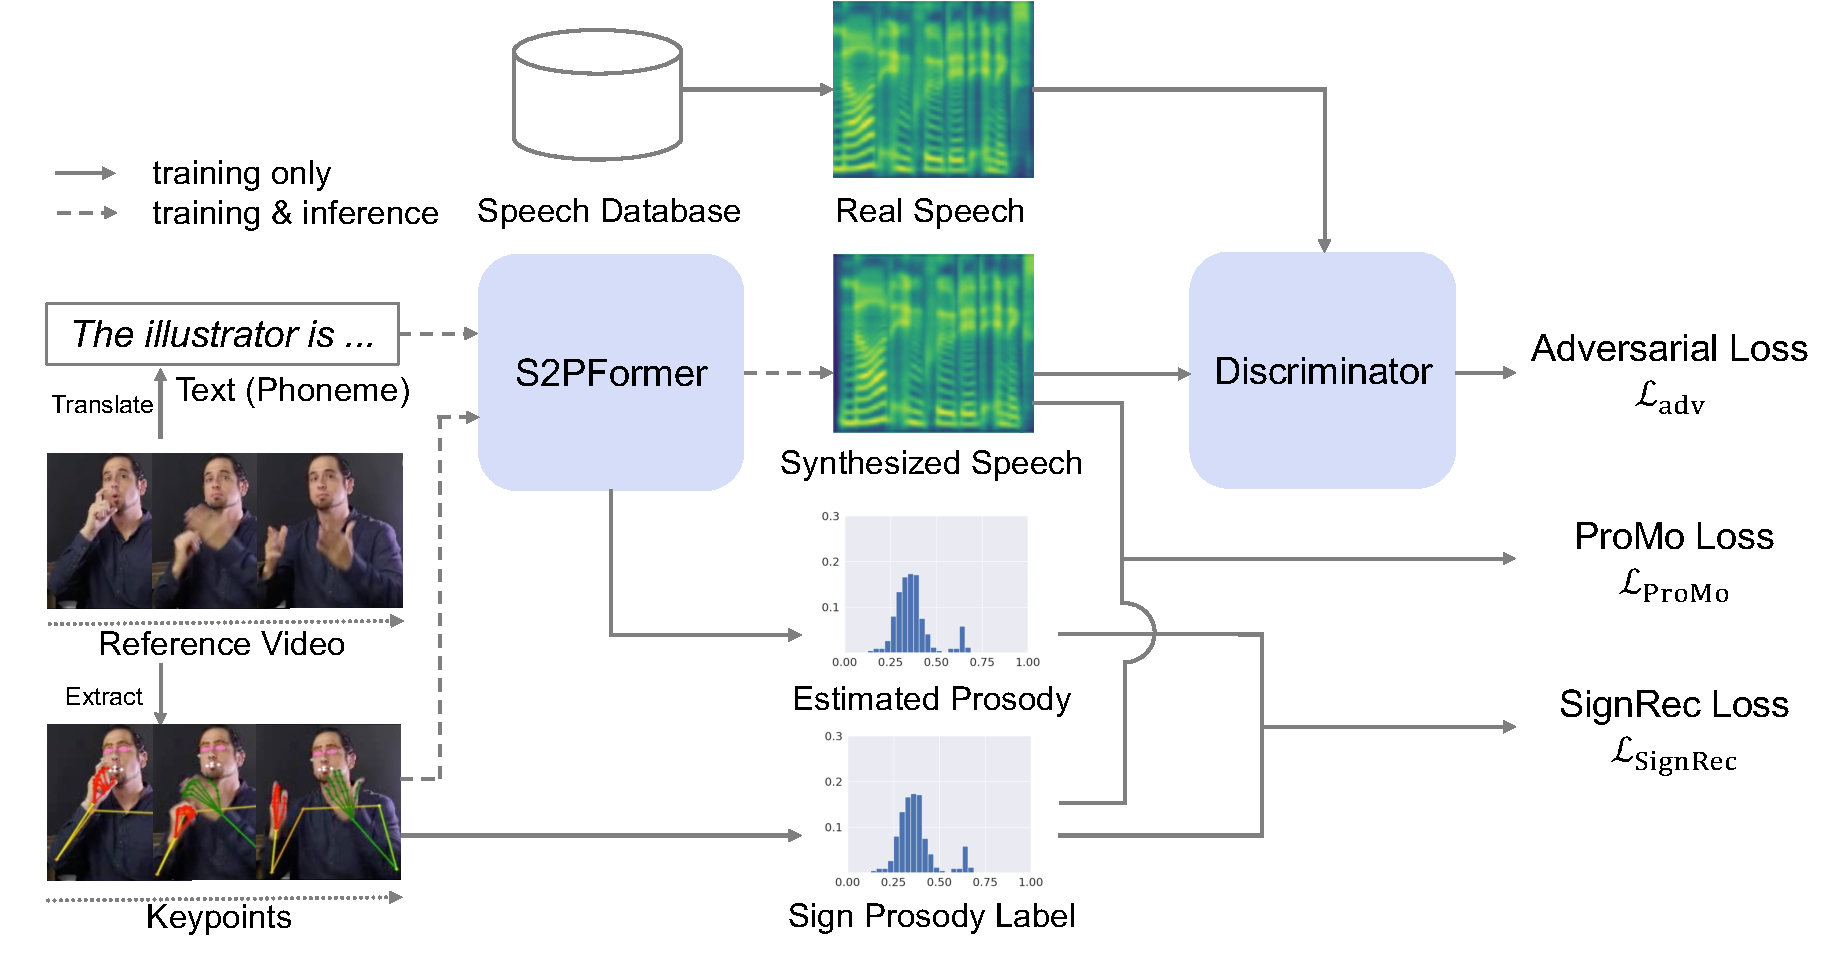
\includegraphics[width=\linewidth]{assets/concept.pdf}}
    \vspace{-2mm}
    \caption{The proposed learning framework of SignRecGAN.}
    \vspace{-4mm}
    \label{fig:overview}
\end{figure}
\manabe{
% アブストの繰り返し, 後で簡略化
We propose a novel task \emph{Sign-to-Speech Prosody Transfer},
aimed at capturing the prosodic nuances conveyed
by sign language and integrating them directly
into speech synthesis.
% global prosody transferであることを定義付ける
% Following prior studies of cross-lingual prosody transfer~\cite{swiatkowski23_interspeech},
% our goal is to transfer global prosody of the source sign.
% ↑までタスクの説明．↓フレームワークの説明
% As the first baseline for this task, we propose \textit{SignRecGAN}.
% following previous work~\cite{swiatkowski23_interspeech}, we adopt an \textit{unpaired} learning framework for \textit{global} prosody transfer
As the first baseline for this task, 
we propose SignRecGAN, a reconstruction- and adversarial-learning framework for prosody-aware speech synthesis. 
By reconstructing motion from the synthesized speech, 
SignRecGAN encourages the synthesized speech to preserve prosodic cues originally expressed in signing.
Adversarial training further promotes naturalness while enabling these prosodic cues to be reflected in a perceptually realistic manner.
% because paired data is difficult to obtain
% as we mentioned in Sec.~\ref{sec:paired_dataset}.
}

As shown in Fig.~\ref{fig:overview}, 
the SignRecGAN has four main components.
First, the S2PFormer (Sec~\ref{sec:ts2s}), our transformer-based model, converts a pair of text and sign language video into speech that reflects sign language prosody.
Next, we introduce SignRec loss (Sec~\ref{sec:prosody_rec}), which reconstructs sign language prosody from the predicted speech. 
Additionally, we introduce ProMo loss (Sec~\ref{sec:PGR}),
a regularization method that leverages prior knowledge about
how speech prosody corresponds to the movements in sign language.
Finally, adversarial learning ensures that the synthesized speech remains realistic (Sec~\ref{sec:training_and_inference}).
% The following subsections describe S2PFormer (Sec.~\ref{sec:ts2s}) and SignRec loss (Sec.~\ref{sec:prosody_rec}). Then, we explain ProMo loss (Sec.~\ref{sec:PGR}).
%-----------------------------------
\begin{figure}[t]
    \centering
    \centerline{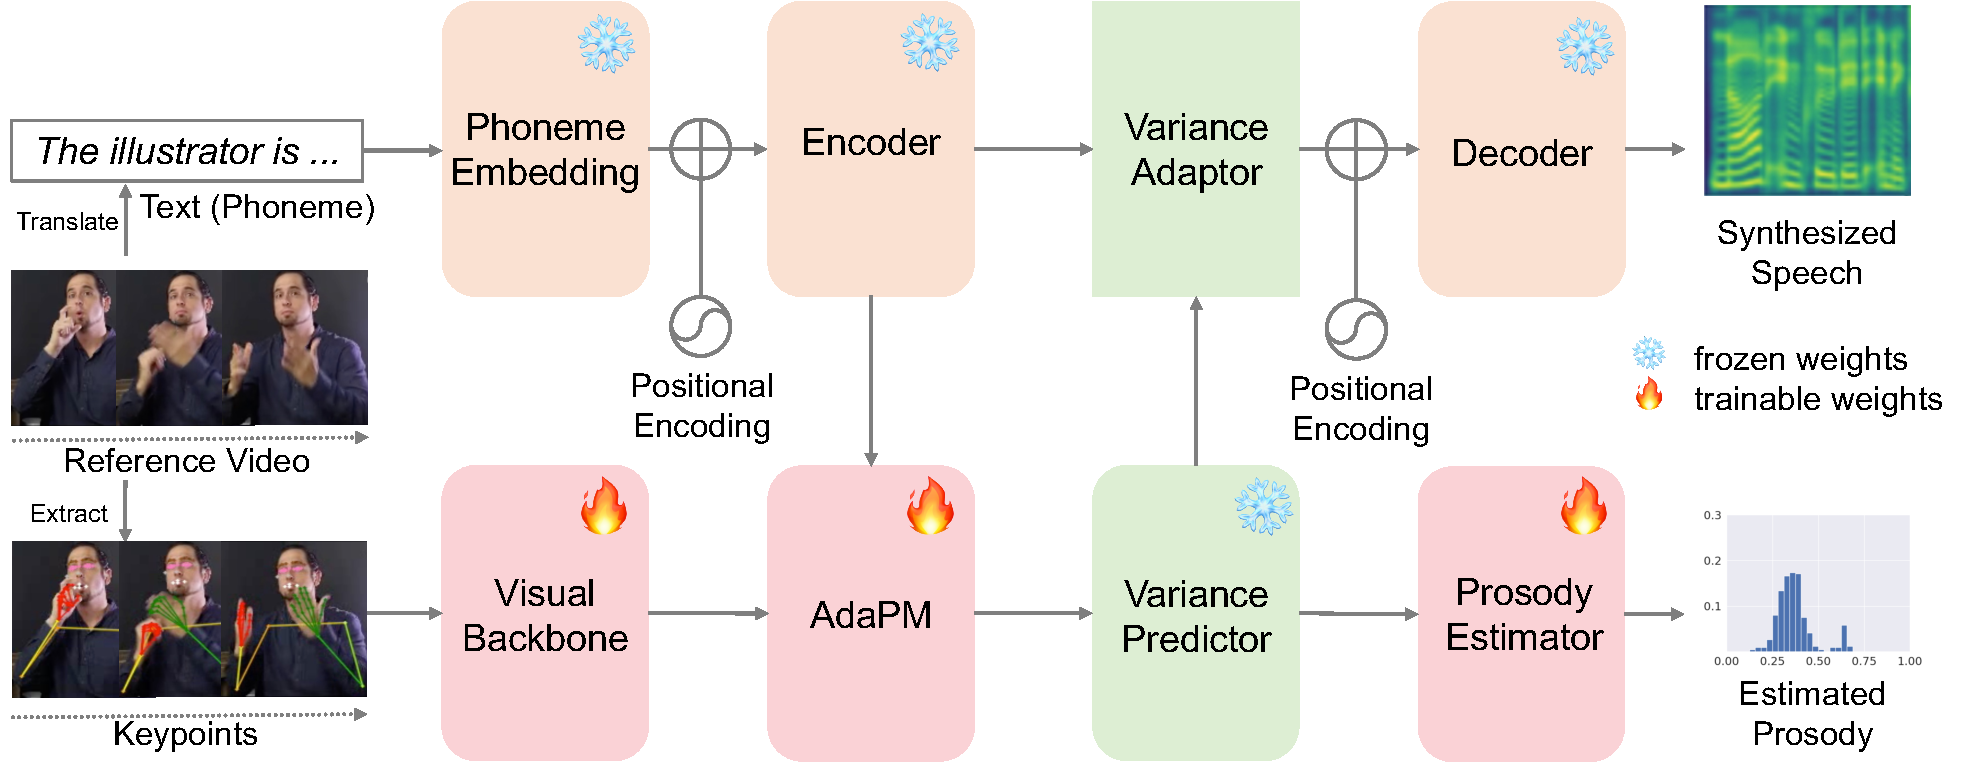
\includegraphics[width=\linewidth]{assets/ts2s.pdf}}
    \vspace{-2mm}
    \caption{The architecture of S2PFormer. S2PFormer extends FastSpeech2 by incorporating sign language information through a module called AdaPM. Specifically, the visual backbone converts sign language inputs into feature representations, which are then fed into AdaPM. Conditioned on these representations, the variance predictor estimates speech prosody parameters, which the prosody estimator uses to predict the original sign language prosody.}
    \vspace{-4mm}
    \label{fig:ts2s}
\end{figure}
\subsection{S2PFormer}
\label{sec:ts2s}
The goal of S2PFormer is to effectively extract prosodic information from sign language and integrate it into speech synthesis to synthesize speech enriched with emotion and emphasis.
This module takes as input a sign language video and its translated text sequence, 
and outputs a mel-spectrogram that reflects the prosody of sign language.
We must preserve the original linguistic content for high-quality speech synthesis. 
% However, linguistic and prosodic information are tightly interrelated, making it challenging to learn both simultaneously. 
% To address this, we leverage pre-trained FastSpeech2.
% We add modules to FastSpeech2 to incorporate sign language information and fine-tune only the modules.
\manabe{
We adopt a pre-trained frozen FastSpeech2~\cite{ren2021fastspeech} backbone to maintain linguistic accuracy. Additionally,  we use a visual backbone, Adaptive Prosody Mixer (AdaPM) and a prosody estimator to incorporate sign language information.
}
% We augment its input with sign language information and fine-tune only the prosody-related modules.
This approach allows us to learn the relationship between sign language and speech prosody without compromising speech quality.
%-----------------------------------

\noindent
\textbf{Preliminaries of text-to-speech synthesis.}
As illustrated in Fig. \ref{fig:ts2s}, a typical FastSpeech2-based module consists of four main components: 
encoder, variance predictor, variance adaptor, and decoder.
Specifically, the encoder first converts a phoneme sequence into phoneme latent representations. 
Then, the variance predictor estimates speech prosody information, pitch, energy and duration, from the phoneme latent representations. 
These predicted prosodic features and phoneme latent representations are passed to the variance adaptor, 
and then processed by the decoder to synthesize a mel-spectrogram.
In the variance adaptor, latent vectors corresponding to pitch and energy are 
first added to phoneme latent representations. 
Then, each element of phoneme latent representations is repeated according to predicted duration.

To incorporate sign language information into speech synthesis, 
we introduce three additional modules: 
visual backbone, Adaptive Prosody Mixer (AdaPM), and prosody estimator.
These components enable the integration of sign language information into speech prosody modeling, enhancing the prosodic naturalness of the synthesized speech.

%-----------------------------------
\noindent{\textbf{Visual Backbone.}}
%-----------------------------------
Sign language is a visual language composed of both motion-based and posture-based expressions.
To extract more abstract features that capture relationships among keypoints and their temporal dynamics, we adopt the keypoint feature extractor from GloFE~\cite{lin-etal-2023-gloss}.
This visual backbone combines CTR-GCN~\cite{Chen_2021_ICCV}, which models keypoint relations as a graph, and MS-TCN~\cite{Liu_2020_CVPR}, which models keypoint positions across frames at multiple temporal resolutions. This backbone transforms sign language keypoints into features.

\begin{figure}[th]
    \centering
    \vspace{-2mm}
    \centerline{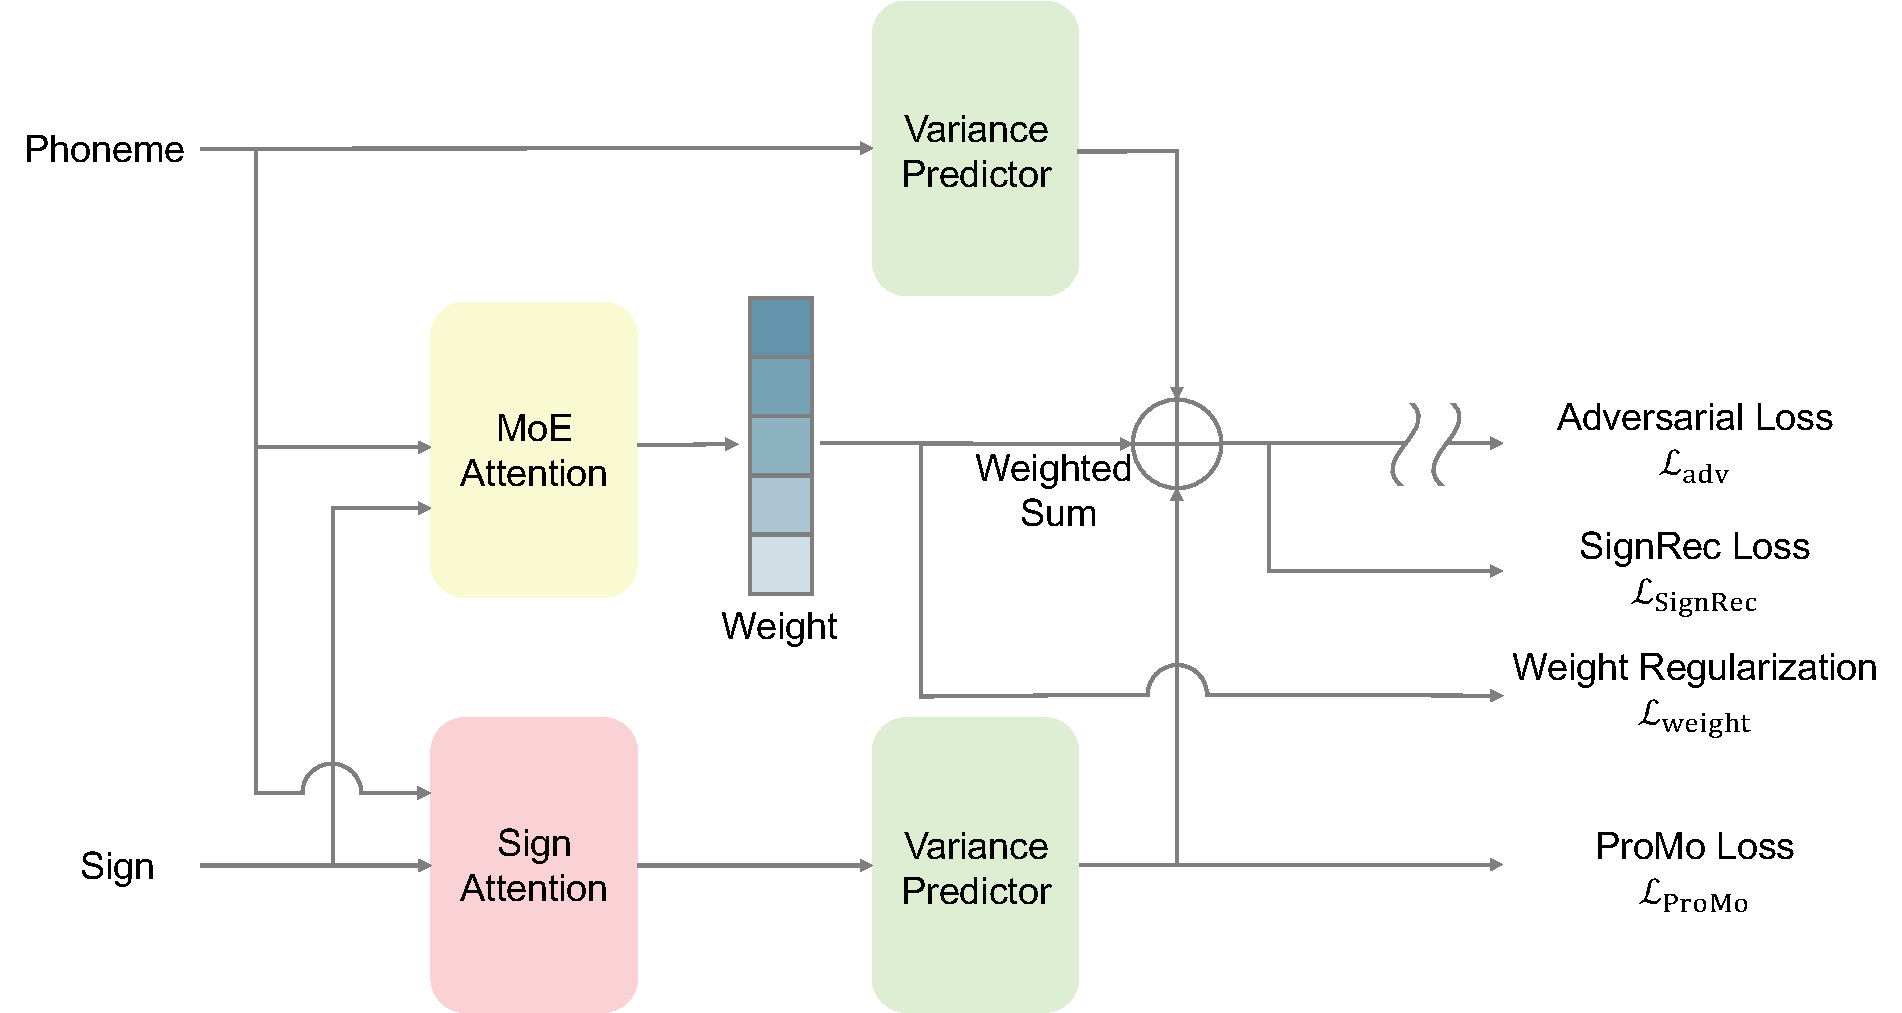
\includegraphics[width=0.8\linewidth]{assets/AdaPM.pdf}}
    \vspace{-2mm}
    \caption{Adaptive Prosody Mixer}
    \label{fig:adapm}
\end{figure}

\noindent{\textbf{Adaptive Prosody Mixer (AdaPM).}}
%-----------------------------------
To reflect sign language information in speech prosody while preserving the speech reality, we introduce AdaPM inspired by Mixture of Experts (MoE)~\cite{shazeer2017outrageouslylargeneuralnetworks}. As shown in Fig.~\ref{fig:adapm}, 
this module adaptively mixes the variance predictions from the phoneme and the sign to balance \manabe{the speech naturalness and the introduced prosody from the reference sign}.
Sign attention and MoE attention are based on the transformer decoder structure~\cite{NIPS2017_3f5ee243}, of which learnable parameters are initialized to zero, 
preventing the speech prosody from becoming noisy at the early stages of training and stabilizing adversarial learning.
Moreover, to avoid the weight for sign language features being too small, we introduce a regularization term defined as follows:
\begin{equation}
    \mathcal{L}_{\mathrm{weight}} = |1 - w_{\mathrm{sign}}|
\end{equation}
where $w_{\mathrm{sign}}$ is the mean of weight for sign language features, and $\lambda_{\mathrm{weight}}$ is a hyperparameter that controls the strength of this regularization.
%-----------------------------------
\begin{figure}[t]
    \centering
    \centerline{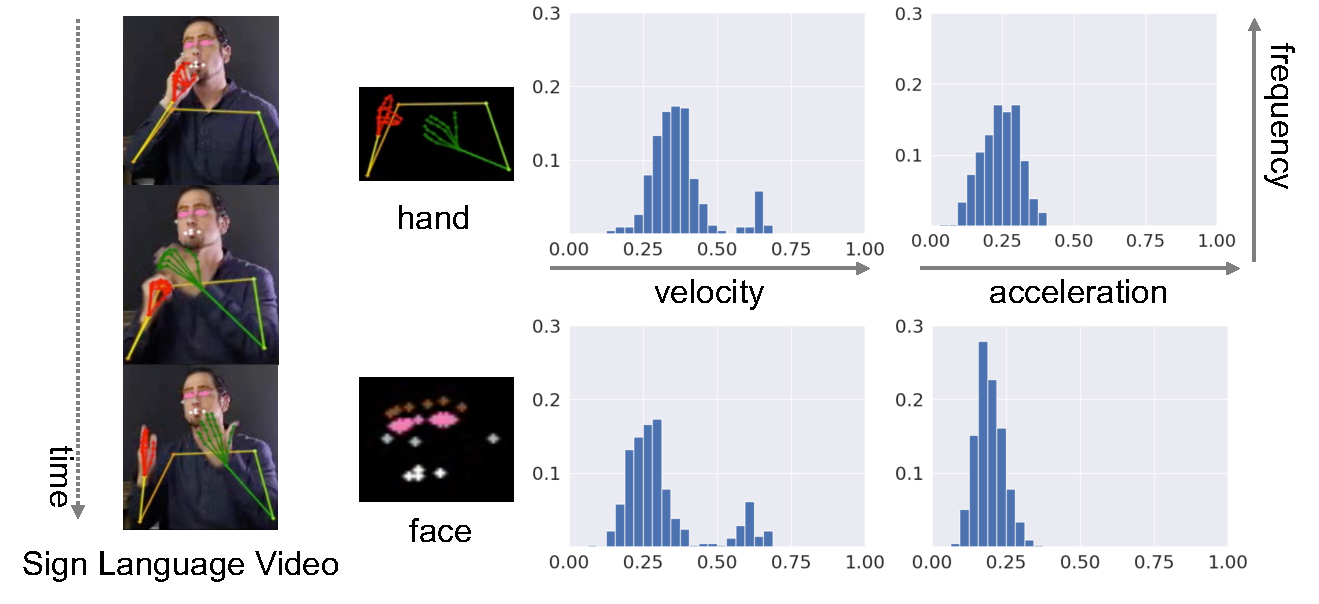
\includegraphics[width=0.8\linewidth]{assets/sign_label.pdf}}
    \vspace{-2mm}
    \caption{An example of sign language prosody labels. The histograms represent the distribution of hand and face motion information in sign language videos.}
    \vspace{-4mm}
    \label{fig:sign_label}
\end{figure}

\subsection{SignRec Loss}
\label{sec:prosody_rec}
%-----------------------------------
To ensure that the speech synthesized by S2PFormer (Sec.~\ref{sec:ts2s}) reflects sign language prosody,
we introduce the SignRec loss, which encourages the prosody estimator to reconstruct sign language prosody from the resulting speech prosody.
If sign language prosody cannot be inferred at all from the speech prosody, 
it indicates there is no correlation between the two.

\noindent
{\textbf{Sign language prosody label.}} In SignRecGAN, 
sign language prosody is defined as the distribution of motion information, 
specifically the velocity and acceleration of representative points of the hands and face in sign language videos (see Fig.~\ref{fig:sign_label}).
To create effective sign language prosody labels, 
we first define the sets of representative points for the hands and face, 
denoted as $\mathcal{H}_{\mathrm{hand}}$ and $\mathcal{H}_{\mathrm{face}}$. 
The velocity $v^i_t=p^i_{t+1}-p^i_t$ and acceleration $a^i_t=v^i_{t+1}-v^i_t$ are then computed for each keypoint $i$. 
\manabe{
To treat each motion information as a scalar value, the squared sum of the values for each representative point set is used,
that is, $V^b_t=\sum_{i\in\mathcal{H}_{b}}\|v^i_t\|^2$, 
$A^b_t=\sum_{i\in\mathcal{H}_{b}}\|a^i_t\|^2$,
$b \in \{\mathrm{hand}, \mathrm{face}\}$. 
}
Let $\mathcal{M}$ be the set of pairs, 
each consisting of a body part and its corresponding motion information. 
For each $M \in \mathcal{M}$, we denote by $M_t$ the squared magnitude of the motion corresponding to $M$ at time $t$.
Next, the squared sums of each motion information are converted into histograms:
\begin{equation}
H_{M}(k)=\sum_{t}\iota(s_k\le M_t <s_{k+1}), s_k=k/S, 0 \le k \le S
\end{equation}
where $\iota(\bullet)$ is an indicator function, and $s_k$ represents the histogram boundaries. The sign language prosody labels are then obtained by normalizing these histograms by the sequence length $T$:
\begin{equation}
P_{M}(k)=\frac{1}{T}H_{M}(k)
\end{equation}

\noindent
{\textbf{Prosody Estimator.}}
The predicted prosody features from the variance predictor, pitch $\hat{p}_{\mathrm{pitch}}$ and energy $\hat{p}_{\mathrm{energy}}$, are concatenated and used as input to estimate the sign language prosody labels $\hat{P}_{M}$. Our SignRec loss, a loss function for the prosody estimator, is defined using cross-entropy loss as follows:
\begin{equation}\label{eq:sign_rec}
\mathcal{L}_{\mathrm{SignRec}}=-\frac{1}{4}\sum_{M \in \mathcal{M}}\sum_{k}P_{M}(k)\log\hat{P}_{M}(k)
\end{equation}
By minimizing this loss, the synthesized speech prosody can reconstruct 
the speed/acceleration variations and shifts in sign language motion,
enabling a more faithful integration 
of sign language prosody into the synthesized speech.


%-----------------------------------
\subsection{ProMo Loss}
\label{sec:PGR}
%-----------------------------------
The learning methods described so far do not rely on paired data, 
meaning that how sign language prosody is reflected in speech prosody remains undetermined. 
To stabilize learning, we introduce cross-modal regularization terms 
based on prior knowledge of prosody in speech and sign language. 
% The prior knowledge includes the correlation between the magnitude of hand movements and the energy of speech, 
% as well as the correlation between the speed of facial movements and the pitch of speech, 
% inspired by the studies about prosody of sign languages and spoken languages~\cite{Wilbur1999,Limousin2010}.
Building on findings in the prosody literature~\cite{Wilbur1999,Limousin2010}, we exploit two correlations: the magnitude of hand movements with speech energy, and the speed of facial movements with speech pitch.
The ProMo loss regularizes prosody by minimizing the L1 distance between speaker-wise standardized speech prosody $\mu_{\mathrm{energy}}, \mu_{\mathrm{pitch}}$ and video-wise standardized sign language prosody $\mu_{v, \mathrm{hand}}, \mu_{v, \mathrm{face}}$,
which is defined as follows:
\begin{equation}\label{eq:pro_mo}
    \mathcal{L}_{\mathrm{ProMo}}=\max\left(\left|\mu_{\mathrm{energy}} - \mu_{v, \mathrm{hand}}\right| - c, 0\right) + \max\left(\left|\mu_{\mathrm{pitch}} - \mu_{v, \mathrm{face}}\right| - c, 0 \right)
\end{equation}
where $c$ is a margin to clip the loss to zero if the two modalities are close enough.

% Consider the case of regularizing speech prosody $m$ and sign language prosody $s$. Here, we specifically discuss regularization based on prior knowledge that $m$ and $s$ have a positive correlation. The loss function is defined by the L1 distance between the means $\mu_m$ and $\mu_s$ of each modality, expressed as $\left|\mu_m - \mu_s\right|$. Each mean is computed after standardizing the respective modality.

% \begin{equation}
%     \mathcal{L}_{\mathrm{ProMo}}=\left|\mu_m - \mu_s\right|
% \end{equation}
%-----------------------------------
\subsection{Training and Inference}
\label{sec:training_and_inference}
%-----------------------------------
In addition to the learning strategies described in Sec.~\ref{sec:prosody_rec} and Sec.~\ref{sec:PGR}, for incorporating sign language prosody into speech, adversarial learning is applied to the synthesized mel-spectrograms to enhance the quality of the synthesized speech. Specifically, the discriminator $\mathcal{D}$ is trained to distinguish whether the input mel-spectrogram is real or synthesized, while the S2PFormer generator $\mathcal{G}$ is trained to deceive the discriminator into classifying synthesized speech as real speech. The adversarial learning loss is designed using the least squares loss from LSGAN~\cite{Mao_2017_ICCV}.
The loss function for the discriminator given a sign language input $X$ and a real speech mel-spectrogram $I$ is defined as follows:
\begin{equation}
    \mathcal{L}_{\mathrm{dis}} = \frac{1}{2}\left(|1 - \mathcal{D}(\mathcal{G}(X))|^2 + |\mathcal{D}(I)|^2\right)
\end{equation}
The adversarial loss given a sign language input $X$ is defined as follows:
\begin{equation}
    \mathcal{L}_{\mathrm{adv}} = |1 - \mathcal{D}(\mathcal{G}(X))|^2
\end{equation}
In addition to adversarial generative loss, to keep synthesized speech more natural, we introduce two regularization terms for synthesized speech: (i) regularization on the intonation, (ii) regularization on speaker likeness. The regularization on the intonation penalizes the synthesized speech if the standard deviation of the pitch and energy, $\sigma_{p}^{g}$ and $\sigma_{e}^{g}$, are smaller than those of the speech synthesized by the two-stage method, $\sigma_{p}^{t}$ and $\sigma_{e}^{t}$. The regularization is defined as follows:
\begin{equation}
    \mathcal{L}_{\mathrm{IR}} = \max(\sigma_{p}^{g} - \sigma_{p}^{t}, 0) + \max(\sigma_{e}^{g} - \sigma_{e}^{t}, 0)
\end{equation}
The regularization on the range of pitch and energy penalizes the synthesized speech if the mean of the pitch and energy, $\mu_{p}^{g}$ and $\mu_{e}^{g}$, fall outside the speaker-specific interval, $\mu_{p}^{\mathrm{speaker}} \pm 3\sigma_{p}^{\mathrm{speaker}}$ and $\mu_{e}^{\mathrm{speaker}} \pm 3\sigma_{e}^{\mathrm{speaker}}$, where $\mu_{p}^{\mathrm{speaker}}, \mu_{e}^{\mathrm{speaker}}, \sigma_{p}^{\mathrm{speaker}}, \sigma_{e}^{\mathrm{speaker}}$ are the mean and standard deviation of pitch and energy. This constraint keeps the overall pitch and energy contours from shifting wholesale, thereby preserving the original speaker’s vocal identity instead of drifting toward a different-sounding voice. The regularization on speaker likeness is defined as follows:
\begin{equation}
    \mathcal{L}_{\mathrm{SL}} = \max(|\mu_{p}^{g} - \mu_{p}^{\mathrm{speaker}}| - 3\sigma_{p}^{\mathrm{speaker}}, 0) + \max(|\mu_{e}^{g} - \mu_{e}^{\mathrm{speaker}}| - 3\sigma_{e}^{\mathrm{speaker}}, 0)
\end{equation}
The generative loss and the regularization terms are summed up as follows:
\begin{equation}\label{eq:natural}
    \mathcal{L}_{\mathrm{natural}} = \mathcal{L}_{\mathrm{adv}} + \lambda_{\mathrm{IR}}\mathcal{L}_{\mathrm{IR}} + \lambda_{\mathrm{SL}}\mathcal{L}_{\mathrm{SL}} 
\end{equation}
where $\lambda_{\mathrm{IR}}$ and $\lambda_{\mathrm{SL}}$ are weight hyperparameters for each loss.

Finally, the generator's loss function is defined as follows:
\begin{equation}
    \mathcal{L} = \mathcal{L}_{\mathrm{natural}}+\lambda_{\mathrm{SignRec}}\mathcal{L}_{\mathrm{SignRec}}+\lambda_{\mathrm{ProMo}}\mathcal{L}_{\mathrm{ProMo}} + \lambda_{\mathrm{weight}} \mathcal{L}_{\mathrm{weight}}
\end{equation}
where $\lambda_{\mathrm{SignRec}}$ and $\lambda_{\mathrm{ProMo}}$ are weights for each loss.

\section{Experiments}
\label{sec:experiments}

\subsection{Experimental Setup}

\subsubsection{Dataset}
\label{subsec:datasets}
As described in Sec~\ref{sec:paired_dataset}, a high-quality dataset that pairs sign language with speech containing prosodic information does not currently exist. Therefore, we train our model using the two unimodal datasets described below.

\noindent{\bf OpenASL}~\cite{shi-etal-2022-open} is a large-scale American Sign Language (ASL) and text dataset collected from YouTube.
It contains diverse situational sign language videos It contains 98,417 translation pairs,
making it one of the largest publicly available ASL translation datasets. 
% In our experiments, we narrowed the set to 16,275 pairs for training simply to examine whether sign prosody is reflected in speech synthesis. 
For our experiments, we subsampled 16,275 pairs for training to evaluate the feasibility of reflecting sign prosody in speech synthesis.
The validation and test sets are composed of 961 and 970 pairs, respectively.

\noindent{\bf VCTK}~\cite{VCTK} is an English speech dataset recorded in a studio by 109 speakers. 
% Each speaker reads different texts; however, some texts are read by multiple speakers. 
We use this dataset as real speech data for adversarial learning.
The total duration of audio exceeds 44 hours, recorded at 48 kHz and converted to 16-bit.

\vspace{-2mm}
\subsubsection{Dataset Preprocessing}
Sign language videos were processed with MMPose~\cite{mmpose} to extract keypoints, and then we clipped the input video frame lengths to be between 30 and 512 frames. To exclude sign language samples with excessively long text, we removed those that deviated by more than 10 standard deviations from the mean.
% The keypoints consist of the wrist, fingertips, elbows, shoulders, and face, yielding $x$ and $y$ coordinates for each part.
For the audio, we used the Montreal Forced Aligner~\cite{mfa} to obtain 80-dimensional mel-spectrograms with a frame size of 1024 and hop size of 256.

\vspace{-2mm}
\subsubsection{Network Details}
Our model is based on FastSpeech2 and was pretrained on VCTK to acquire speaker information. We utilized open-source implementations of FastSpeech2\footnote{\url{https://github.com/ming024/FastSpeech2}} and the Visual Backbone\footnote{\url{https://github.com/HenryLittle/GloFE}}.
% The Prosody Estimator is composed of an FCN and prediction heads for each prosody label.
We trained our model on 3 NVIDIA RTX A5000 GPUs with a per-GPU batch size of 10.
For the optimization method, we used AdamW~\cite{loshchilov2018decoupled} for all models. For more details regarding hyper parameters and model implementation, please refer to the Appendix.

\vspace{-2mm}
\subsubsection{Evaluation Method}
In this paper, we evaluate the quality of synthesized speech using both objective and subjective assessments.
For the objective evaluation, 
we measure the expressiveness and naturalness of synthesized speech. 
For subjective evaluation, 
we conduct a user study and report comparative mean opinion scores (CMOS),
\manabe{following previous work of cross-lingual prosody transfer~\cite{swiatkowski23_interspeech}.}

\noindent{\bf Expressiveness}
To measure the richness of emotional expression in speech,
we calculate the standard deviations of predicted pitch and energy contours. 
Larger standard deviations indicate richer emotional expression~\cite{kharitonov-etal-2022-text}.
To evaluate the overall speech quality, 
we calculate the standard deviation across the test set, 
and to evaluate individual samples, 
we calculate the standard deviation for each speech sample and then take the mean of these values.

\noindent{\bf Naturalness}
To evaluate the quality of the synthesized speech and to show that our model does not degrade the quality of the speech, 
we use WER (Word Error Rate) and UTMOS\footnote{\url{https://github.com/sarulab-speech/UTMOS22}}~\cite{saeki22c_interspeech}. 
We use the pretrained automatic speech recognition model, 
Whisper large V3\footnote{\url{https://huggingface.co/openai/whisper-large-v3}}~\cite{radford2022whisper} to calculate WER. 
In particular, some text translations in OpenASL are inappropriate for speech synthesis: too long texts or too rare vocabularies. 
Therefore, we filtered out the text longer than 18 words and the text containing words of three or more capital letters.

\noindent{\bf User Study}
% We conducted a CMOS test to compare the two-stage method with the proposed method in how well the synthesized speech matches the source sign language prosody and naturalness. 
\manabe{
We conducted a CMOS test to evaluate how well and naturally
the synthesized speech matches the source sign language prosody. 
}
We grouped samples into three categories based on text length: Short (3-8 words), Medium (9-13 words), and Long (14-18 words). 
In addition, we categorized the 30 sign language videos with the lowest mean facial velocity as Neutral. 
% When the sign language contains low prosody, 
% the two-stage method can still produce speech with adequate prosody. 
% Therefore, on low prosody samples, 
% SignRecGAN should simply avoid degrading speech quality.
Given that the two-stage approach yields sufficient prosody, SignRecGAN's primary role in these cases is to maintain baseline speech quality without introducing artifacts.
In the CMOS test, 17 participants\footnote{A participant accidentally took the two types of tests.} rated each sample on a five grade evaluation.
Please refer to the Appendix for more details on the user study.

\noindent{\bf Prominence Analysis}
While our proposed method primarily focuses on reconstructing global prosody, it is crucial to verify whether this also results in high-quality, fine-grained prosodic features. 
To this end, we conducted a prominence analysis using the Wavelet Prosody Toolkit\footnote{\url{https://github.com/asuni/wavelet_prosody_toolkit}}~\cite{DBLP:journals/corr/SuniAV15}. For a more detailed explanation of prominence analysis,
please refer to the Appendix.

\begin{table}[t]\fontsize{10pt}{10pt}\selectfont
    \centering
    \caption{Objective evaluation. 
    % Expressiveness is considered better the closer its values to those of real speech. 
    The best scores are highlighted in \textbf{bold}, and the second-best scores are \underline{underlined}.}
    \label{tab:objective}
    \vspace{-3mm}
    \begin{tabular}[t]{lccccccc}
    \toprule
      &&&& \multicolumn{2}{c}{Expressiveness} & \multicolumn{2}{c}{Naturalness} \\
    Method & $\mathcal{L}_{\mathrm{natural}}$ & $\mathcal{L}_{\mathrm{SignRec}}$ & $\mathcal{L}_{\mathrm{ProMo}}$ & Pitch($\rightarrow$) & Energy($\rightarrow$) & WER($\downarrow$) & UTMOS($\uparrow$) \\
    \midrule
    Real Speech &  &  &  & 28.9 & 25.4 & 0.04 & 4.07 \\
    \midrule
    two-stage &  &  &  & \underline{17.6} & 20.1 & \underline{0.293} & \textbf{3.52} \\
    \midrule
    \multirow{4}{*}{Ours} & \Checkmark &  &  & 48.4 & 44.6 & \textbf{0.212} & 3.29 \\
     & \Checkmark & \Checkmark &  & 44.2 & 39.7 & 0.448 & 2.95 \\
     & \Checkmark &  & \Checkmark   & 45.3 & \underline{28.6} & 0.623 & 3.03 \\
     & \Checkmark & \Checkmark & \Checkmark                  & \textbf{33.7} & \textbf{22.5} & 0.325 & \underline{3.44}\\
    \bottomrule
    \end{tabular}
    \vspace{-4mm}
\end{table}


\subsection{Objective Evaluation}
Table~\ref{tab:objective} shows the result of comparing the expressiveness of the synthesized speech and that of real speech. 
As can be seen, SignRecGAN exhibits higher expressiveness values for pitch and energy than the two-stage method, 
and these values are closer to those of real speech. 
This suggests that intonation and emphasis similar to real speech can be achieved more effectively than with the two-stage method, 
although SignRecGAN slightly degrades the naturalness of the synthesized speech compared to the two-stage method.

\subsection{Ablation Study}
To investigate the effectiveness of each component in SignRecGAN, we conducted an ablation study.
GAN, SignRec, and ProMo indicate the S2PFormer with the losses defined in Eqs.~\ref{eq:natural}, \ref{eq:sign_rec}, \ref{eq:pro_mo} respectively.
The result in Table~\ref{tab:objective} show that every component alone does not contribute to improvement of expressiveness, and the combination of all three components is necessary to achieve the best performance. 
In particular, our ablation shows that 
if either the SignRec loss or the ProMo loss is removed, 
naturalness degrades even with the adversarial loss, 
indicating that all three components are necessary to maintain natural-sounding speech.
% Especially, the combinations of GAN with SignRec loss and with ProMo loss show significant degradation in naturalness.

\begin{table}[t]
    \centering
    \caption{The CMOS of the user study with 95\% confidence intervals. The scores with statistically significant improvements are highlighted in \colorbox{lightgreen}{green}.}
    \vspace{-2mm}
    \begin{tabular}{l c c c c c}
        \toprule
         & Short & Medium & Long & Neutral & Total \\
        \midrule
        Prosody & $3.12 (\pm 0.22)$ & \cellcolor{lightgreen}$3.19 (\pm 0.16)$ & \cellcolor{lightgreen} $3.19 (\pm 0.16)$ & $3.00 (\pm 0.18)$ & \cellcolor{lightgreen} $3.17 (\pm 0.11)$ \\
        Naturalness & $2.93 (\pm 0.17)$ & $2.97 (\pm 0.17)$ & $2.87 (\pm 0.15)$ & $2.96 (\pm 0.15)$ & $2.92 (\pm 0.11)$ \\
        \bottomrule
    \end{tabular}
    \label{tab:user_study}
    \vspace{-2mm}
\end{table}


\subsection{User Study}
Table~\ref{tab:user_study} shows that SignRecGAN produced results more consistent with sign language prosody than the two-stage method. In particular, the results for the Medium and Long categories show statistically significant differences, whereas the two methods do not differ significantly in naturalness.
Taken together with the quantitative evaluation results, these results indicate a slight degradation in naturalness.
Also, the scores for Neutral category did not show a statistically significant difference, indicating that SignRecGAN does not degrade the quality of synthesized speech.

\begin{figure}[t] %{0.6\textwidth}
    \centering
    \centerline{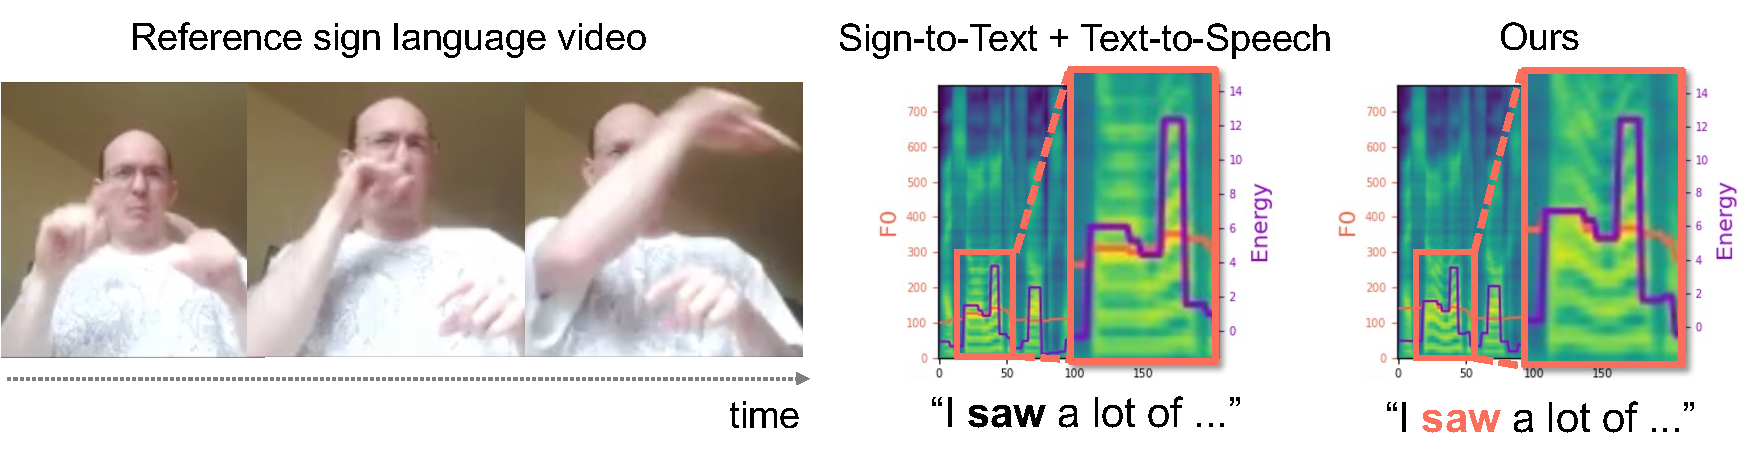
\includegraphics[width=\linewidth]{assets/mel_vis1.pdf}}
    \vspace{-4mm}
    \caption{An example of input sign language video (left) and synthesized speech (right).}
    \vspace{-2mm}
    \label{fig:mel_ex1}
\end{figure}


\subsection{Qualitative Evaluation}
\label{sec:qualitative}
Fig.~\ref{fig:mel_ex1} presents an example of the synthesized speech, one of the highest scored samples in the user study. In the reference sign language video, the signer signs the phrase ``I saw'' with dynamic facial expressions and hand movements. SignRecGAN successfully represents the emphasis on the phrase, while two-stage method fails.

\begin{figure}[th]
    \centering
    \centerline{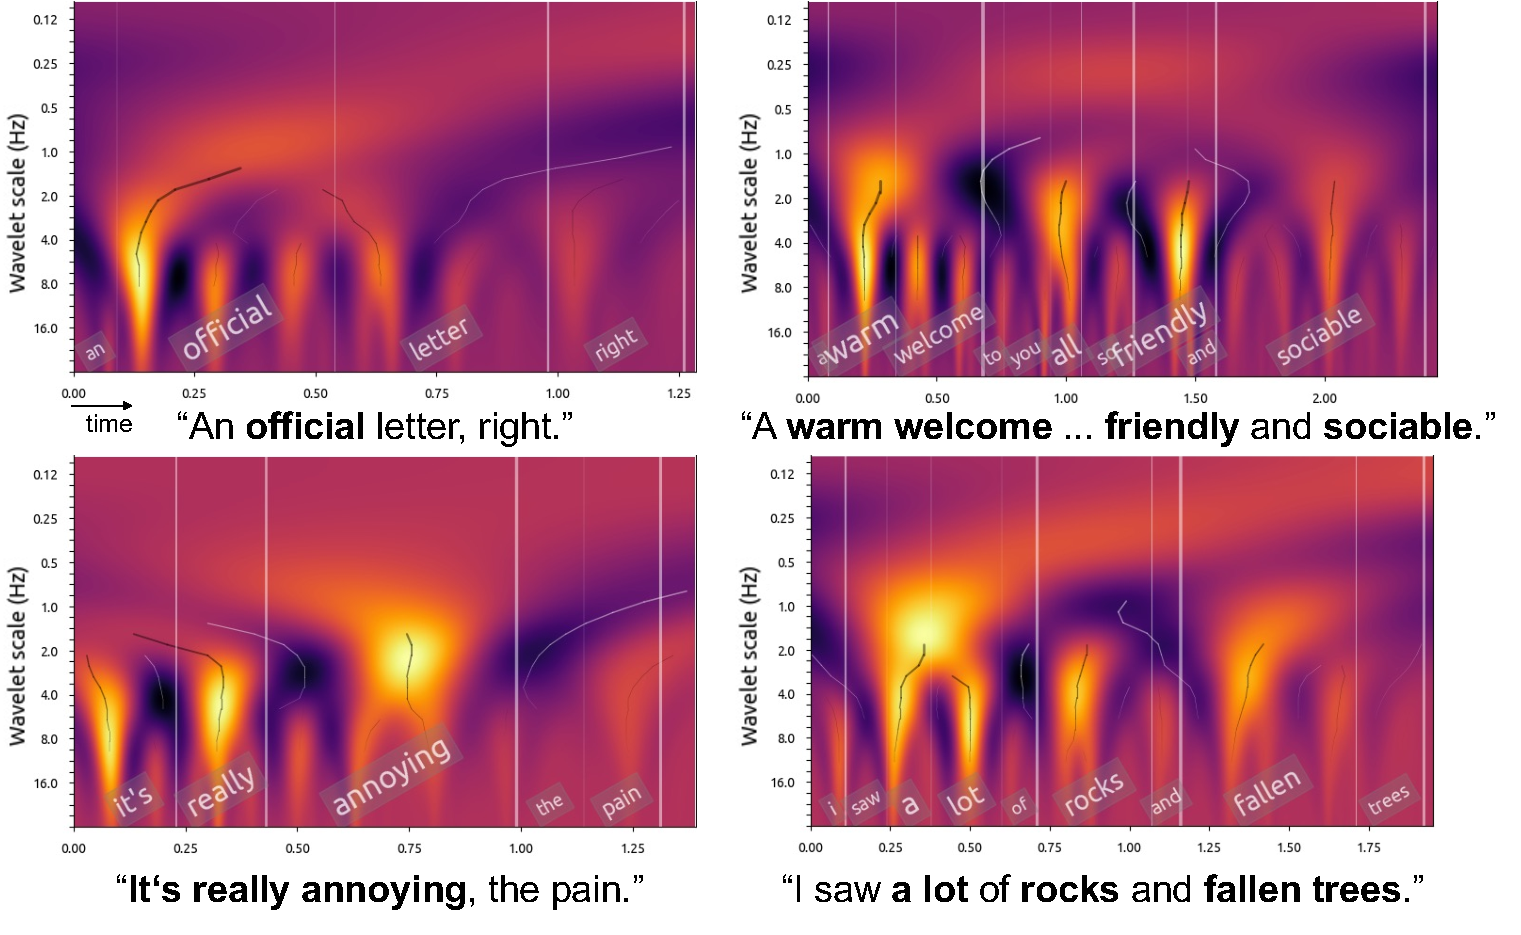
\includegraphics[width=\linewidth]{assets/prominence.pdf}}
    \vspace{-2mm}
    \caption{Prominence analysis results. A black line on a spectrogram indicates emphasis, and the corresponding word is labeled on the spectrogram. The size of a labeled word indicates the intensity of the emphasis.}
    \label{fig:prominece}
    \vspace{-6mm}
\end{figure}

\subsection{Emergence of Emphasis on Natural Words}
\manabe{
Regarding to fine-grained prosody evaluation, Fig.~\ref{fig:prominece} shows some results of prominence analysis~\cite{DBLP:journals/corr/SuniAV15}.
The results indicate that S2PFormer can emphasize suitable words (e.g., ``\textit{annoying}'', ``\textit{a lot}'') and does not emphasize unnatural words (e.g., ``\textit{and}'').
% It is considered to be realized by adversarial learning.
% Therefore, even though SignRecGAN relies on global prosody,
% the synthesized speeches are natural.
This suggests that while the reconstruction loss facilitates the modeling of global prosody, its combination with adversarial learning enables the model to selectively emphasize contextually natural words.
}

% Fig.~\ref{fig:mel_ex2} presents another example of synthesized speech. In this case, the sign language speaker displays particularly expressive facial expressions alongside large, pronounced signing movements. Correspondingly, the resulting speech shows a global increase in both energy and pitch. However, one limitation of the speech synthesized by the proposed method is that the pitch remains nearly constant, leading to an absence of natural intonation. This suggests that, although the ProMo loss effectively aligned the mean values of prosodic features, the SignRec loss may not have been sufficiently trained to capture the overall shape of their distribution.

% \begin{figure}[t]
%     \centering
%     \centerline{\includegraphics[width=0.3\linewidth]{images/melspec/ex2.pdf}}
%     \caption{The reference sign language video and the synthesized speeches of ``Sadly some children never get adopted.''.}
%     \vspace{-2mm}
%     \label{fig:mel_ex2}
% \end{figure}
% \subsection{Limitations}
% \noindent{\bf Emotion understanding:} Because our proposed sign language prosody labels just incorporate lower level metrics such as velocity and acceleration, they may not adequately capture higher level attributes like emotion. We will investigate modeling incorporating richier emotional informatino in future work.

% \noindent{\bf Quantitative evaluation:} Since there is not existing method to measure how the prosody of synthesized speech matches that of sign language, we have to rely on limited aspect of model performance.

\section{Conclusion}
\label{sec:conclusion}
In this study, we tackled a novel task \emph{Sign-to-Speech Prosody Transfer}, 
which seeks to transfer sign language prosody into synthesized speech. 
\manabe{
% This task poses multiple challenges, 
% including the lack of a high-quality dataset that aligns sign language with speech, 
% and the extremely complex correspondence between the two modalities.
The major challenge for this task is the lack of datasets that align sign and speech.
Constructing such datasets requires expert knowledge, making annotation extremely costly.
To address this challenge, 
we introduce \emph{SignRecGAN}, 
a training framework utilizing unimodal datasets of speech and sign language 
through adversarial learning and reconstruction loss.
}
% we proposed a learning framework that utilizes unpaired unimodal datasets of speech and sign language.
% Our approach combines prosody reconstruction and regularization grounded in prior knowledge of prosody. 
Through quantitative evaluation and user studies, 
we demonstrated that the proposed method can produce speech 
that better reflects the sign language prosody.
% \noindent{\bf Limitations}

% \noindent{\bf Quantitative evaluation:} Since there is no existing method to measure how the prosody of synthesized speech matches that of sign language, we have to rely on a limited set of performance aspects.

% \noindent{\bf Emotion understanding:} Because our proposed sign language prosody labels only incorporate lower level metrics such as velocity and acceleration, they may not adequately capture higher level attributes like emotion. We will investigate modeling incorporating richer emotional information in future work.

%
%
%
% \section{First Section}
% \subsection{A Subsection Sample}
% Please note that the first paragraph of a section or subsection is
% not indented. The first paragraph that follows a table, figure,
% equation etc. does not need an indent, either.

% Subsequent paragraphs, however, are indented.

% \subsubsection{Sample Heading (Third Level)} Only two levels of
% headings should be numbered. Lower level headings remain unnumbered;
% they are formatted as run-in headings.

% \paragraph{Sample Heading (Fourth Level)}
% The contribution should contain no more than four levels of
% headings. Table~\ref{tab1} gives a summary of all heading levels.

% \begin{table}
% \caption{Table captions should be placed above the
% tables.}\label{tab1}
% \begin{tabular}{|l|l|l|}
% \hline
% Heading level &  Example & Font size and style\\
% \hline
% Title (centered) &  {\Large\bfseries Lecture Notes} & 14 point, bold\\
% 1st-level heading &  {\large\bfseries 1 Introduction} & 12 point, bold\\
% 2nd-level heading & {\bfseries 2.1 Printing Area} & 10 point, bold\\
% 3rd-level heading & {\bfseries Run-in Heading in Bold.} Text follows & 10 point, bold\\
% 4th-level heading & {\itshape Lowest Level Heading.} Text follows & 10 point, italic\\
% \hline
% \end{tabular}
% \end{table}


% \noindent Displayed equations are centered and set on a separate
% line.
% \begin{equation}
% x + y = z
% \end{equation}
% Please try to avoid rasterized images for line-art diagrams and
% schemas. Whenever possible, use vector graphics instead (see
% Fig.~\ref{fig1}).

% \begin{figure}
% 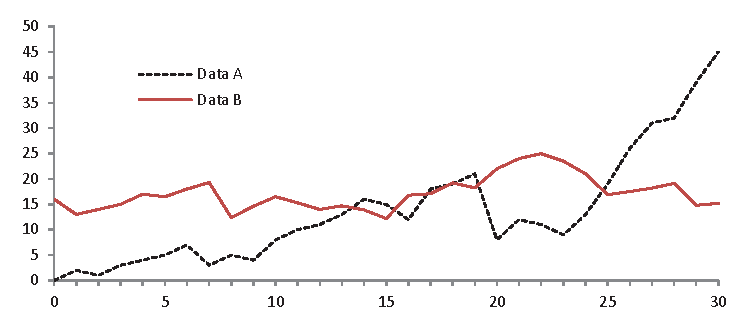
\includegraphics[width=\textwidth]{fig1.eps}
% \caption{A figure caption is always placed below the illustration.
% Please note that short captions are centered, while long ones are
% justified by the macro package automatically.} \label{fig1}
% \end{figure}

% \begin{theorem}
% This is a sample theorem. The run-in heading is set in bold, while
% the following text appears in italics. Definitions, lemmas,
% propositions, and corollaries are styled the same way.
% \end{theorem}
% %
% % the environments 'definition', 'lemma', 'proposition', 'corollary',
% % 'remark', and 'example' are defined in the LLNCS documentclass as well.
% %
% \begin{proof}
% Proofs, examples, and remarks have the initial word in italics,
% while the following text appears in normal font.
% \end{proof}
% For citations of references, we prefer the use of square brackets
% and consecutive numbers. Citations using labels or the author/year
% convention are also acceptable. The following bibliography provides
% a sample reference list with entries for journal
% articles~\cite{ref_article1}, an LNCS chapter~\cite{ref_lncs1}, a
% book~\cite{ref_book1}, proceedings without editors~\cite{ref_proc1},
% and a homepage~\cite{ref_url1}. Multiple citations are grouped
% \cite{ref_article1,ref_lncs1,ref_book1},
% \cite{ref_article1,ref_book1,ref_proc1,ref_url1}.

% \subsubsection{Acknowledgements} Please place your acknowledgments at
% the end of the paper, preceded by an unnumbered run-in heading (i.e.
% 3rd-level heading).

% %
% % ---- Bibliography ----
% %
% % BibTeX users should specify bibliography style 'splncs04'.
% % References will then be sorted and formatted in the correct style.
% %
% % \bibliographystyle{splncs04}
% % \bibliography{mybibliography}
% %
% \begin{thebibliography}{8}
% \bibitem{ref_article1}
% Author, F.: Article title. Journal \textbf{2}(5), 99--110 (2016)

% \bibitem{ref_lncs1}
% Author, F., Author, S.: Title of a proceedings paper. In: Editor,
% F., Editor, S. (eds.) CONFERENCE 2016, LNCS, vol. 9999, pp. 1--13.
% Springer, Heidelberg (2016). \doi{10.10007/1234567890}

% \bibitem{ref_book1}
% Author, F., Author, S., Author, T.: Book title. 2nd edn. Publisher,
% Location (1999)

% \bibitem{ref_proc1}
% Author, A.-B.: Contribution title. In: 9th International Proceedings
% on Proceedings, pp. 1--2. Publisher, Location (2010)

% \bibitem{ref_url1}
% LNCS Homepage, \url{http://www.springer.com/lncs}. Last accessed 4
% Oct 2017
{
    \small
    \bibliographystyle{splncs04}
    \bibliography{main}
}
\end{document}
